\documentclass[14pt, a4paper]{article}

\usepackage[utf8]{inputenc}
\usepackage[T2A]{fontenc}

\usepackage{graphicx}
\graphicspath{ {images/} }

\usepackage{amsmath}
\usepackage{mathtext}
\usepackage{fontenc}


\title{Курсовая работа по электротехнике. Часть 2}
\author{Новоженов П.А. ЭН-26}
\date{}

\begin{document}

    \maketitle

    \newpage

    \section*{Цель работы}
        Исследование сложной цепи синусоидального тока посредством комплексных
        чисел и векторных диаграмм

    \section*{Рассчет цепи}

    $$\omega = 2\pi f = 18840 \frac{\text{рад}}{\text{с}}$$


    $$Z_S = \sqrt{(\omega L - \frac{1}{\omega C})^2} = 18840 \cdot 0.6 \cdot 10^{-3} - \frac{1}{18840 \cdot 5 \cdot 10^{-6}} = 0.69 \ \text{Ом}$$
    $$\overline{Z_S} = j(\omega L - \frac{1}{\omega C}) = 0.69j = 0.69e^{i90^\circ \ \text{Ом}}$$

    $$\overline{Y_{P_2}} = \frac{1}{R} + j\frac{1}{\omega L} = 0.16 + 0.26j = 0.31e^{i58^\circ}\ \text{См}$$

    $$\overline{Y_{P_3}} = \frac{1}{R} + j\omega C = 0.1 + 0.09j = 0.13e^{i41^\circ}\ \text{См}$$

    $$\overline{Z_{P_2}} = \frac{1}{\overline{Y_{P_2}}} = 3.28e^{-58^\circ i} \ \text{Ом}$$

    $$\overline{Z_{P_2}} = \frac{1}{\overline{Y_{P_3}}} = 7.43e^{-41^\circ i} \ \text{Ом}$$

    Найдем суммарное сопротивление $P_2$ и $P_3$:
    $$Y_P = \overline{Y_{P_2}} + \overline{Y_{P_3}} = 0.31e^{i58^\circ} + 0.13e^{i83^\circ} = 0.44 e^{i53^\circ}\ \text{См}$$
    $$Z_P = \frac{1}{\overline{Y_P}} = 2.29 e^{-53^\circ i} \ \text{Ом}$$

    Найдем сопротивление нагрузки:
    $$\overline{Z_o} = Z_P + Z_S = 2.29e^{-53^\circ i} + 0.69e^{i90^\circ} = 1.79 e^{-40^\circ i} \ \text{Ом}$$

    Найдем:
    $$\overline{I_1} = \frac{\overline{E}}{\overline{Z_o}} = \frac{8e^{i0^\circ}}{1.79 e^{-40^\circ i}} = 4.48 e^{40^\circ i} \ \text{A}$$
    $$\overline{U_1} = \overline{I_1} \cdot \overline{Z_S} = 3.09 e^{-49^\circ i} \ \text{В}$$
    $$\overline{U2} = \overline{I_1} \cdot \overline{Z_P} = 10.26 e^{-13^\circ i} \ \text{В}$$
    $$\overline{I_2} = \frac{\overline{U2}}{\overline{Z_2}} = 3.13 e^{45^\circ i} \ \text{A}$$
    $$\overline{I_3} = \frac{\overline{U_2}}{\overline{Z_3}} = 1.38 e^{28^\circ i} \ \text{A}$$

    $$\varphi_1 = 90^\circ$$
    $$\varphi_2 = asin(\frac{X_{P_2}}{Z_{P_2}}) = 57^\circ$$
    $$\varphi_3 = asin(\frac{X_{P_3}}{Z_{P_3}}) = 43^\circ$$
    $$\varphi = asin(\frac{X}{Z}) = 57^\circ$$

    Изобразим векторную диаграмму:

    {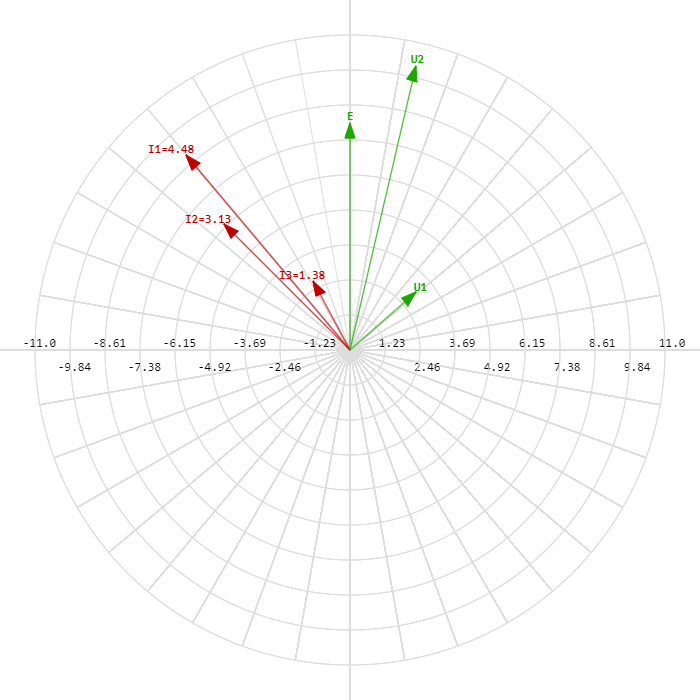
\includegraphics[width=0.9\textwidth]{diag1.png}}


    \section*{Результат моделирования}

    {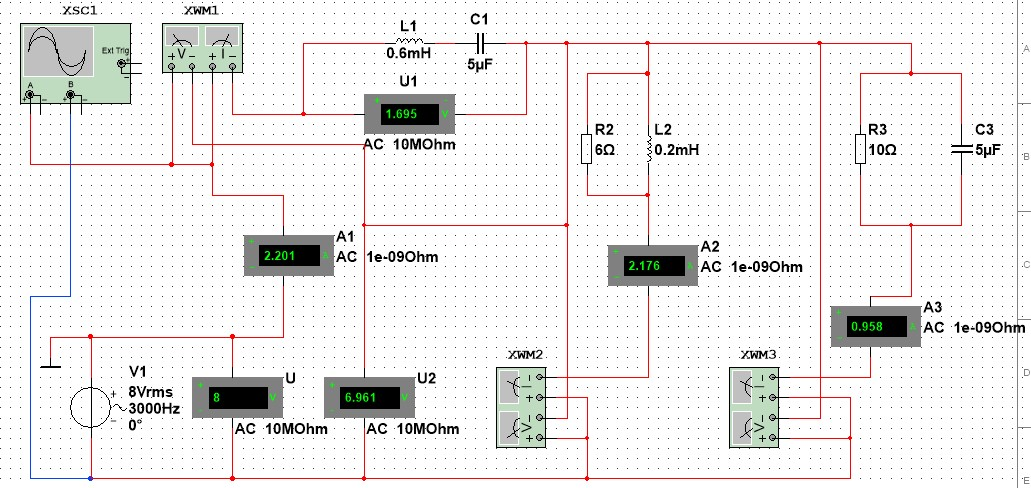
\includegraphics[width=1\textwidth]{design1.jpg}}

    По результату моделирования заполним таблицу:

    {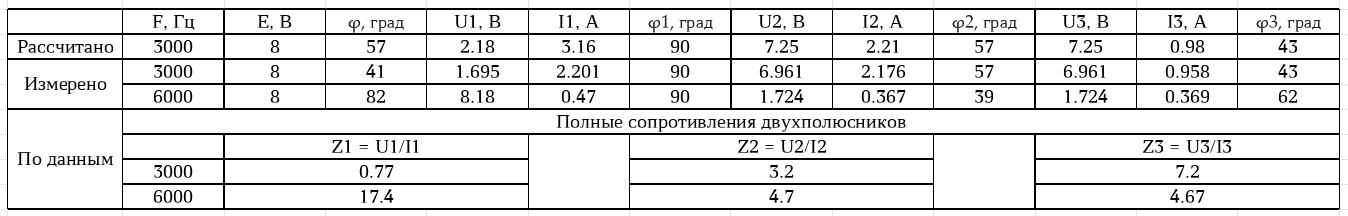
\includegraphics[width=1\textwidth]{table.jpg}}

    Изобразим треугольники сопротивлений. Для сопротивления $Z_1$ при $f=6000$ я не стал изображать треугольник сопротивления, так как он представляет собой прямую, причем
    сильно выбивающуюся из размеров остальных треугольников. 

    {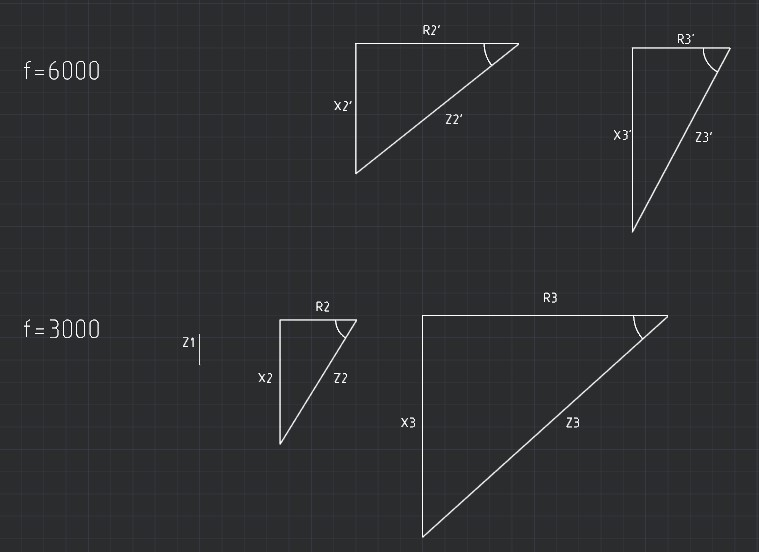
\includegraphics[width=1\textwidth]{triangles.jpg}}

    \section*{Вывод работы}
        В ходе данной работы мы исследовали сложную цепь синусоидального тока посредством комплексных чисел и векторных диаграмм.

    

\end{document}